%% =====================================================================
%% Documento de Planejamento do Projeto — Entrega 01 (29/08/2026)
%% Experiência Criativa: Projeto Transformador II — BCC / PUCPR
%% Autora: Gabriela Sofia
%% Formatação: IEEEtran conference (padrão do template dos professores)
%% Compilar: pdflatex main && pdflatex main
%% Versão: v2 (2026-08-11) — reescrita com o estado da frente externa
%% =====================================================================
\documentclass[conference]{IEEEtran}
\IEEEoverridecommandlockouts

\usepackage[T1]{fontenc}
\usepackage[utf8]{inputenc}
\usepackage[brazil]{babel}
\usepackage{graphicx}
\usepackage{booktabs}
\usepackage{array}
\usepackage{amsmath,amssymb}
\usepackage{xcolor}
\usepackage{tikz}
\usetikzlibrary{arrows.meta,positioning,fit,backgrounds,shapes.misc}
\usepackage{cite}
\usepackage{url}
\usepackage[hidelinks]{hyperref}

% cores do diagrama
\definecolor{cAzul}{HTML}{1F4E79}
\definecolor{cVerm}{HTML}{C0504D}
\definecolor{cVerd}{HTML}{3F6F4A}
\definecolor{cCinz}{HTML}{7F7F7F}
\definecolor{cFundo}{HTML}{EEF3F8}
\definecolor{cFundoAux}{HTML}{F7F0EE}
\definecolor{cFundoPrd}{HTML}{EDF3EE}

\begin{document}

\title{Onde a água chega primeiro: suscetibilidade urbana a enchentes
com variáveis físico-hidrológicas interpretáveis e negativo observado}

\author{\IEEEauthorblockN{Gabriela Sofia}
\IEEEauthorblockA{Experiência Criativa: Projeto Transformador II\\
Bacharelado em Ciência da Computação --- PUCPR\\
Turma \textcolor{red}{7A} --- Equipe \textcolor{red}{N}\\
\{\texttt{gabriela.milani}\}@pucpr.edu.br}}

\maketitle

% =====================================================================
\section{Descrição do Projeto}

A chuva cai sem escolher; a água, depois de cair, escolhe. Ela desce pelo
terreno até o ponto mais baixo, e o ponto mais baixo da cidade brasileira
costuma ser onde mora quem não teve escolha sobre onde morar. Entre 2000 e 2018
a população exposta a inundação cresceu dez vezes mais do que as projeções
previam, concentrada onde a ocupação já era precária~\cite{tellman2021}. No Brasil
soma-se uma desigualdade de registro: o evento entra nos dados por quem atende a
emergência --- Defesa Civil, canal 156, decreto municipal ---, de modo que o
dado descreve o atendimento, e não a água. Bairro sem chamado não é bairro seco.

O fenômeno físico é simples de enunciar: há enchente quando chega a um ponto
mais água do que ele consegue escoar ou armazenar. Isso se decompõe em três
grandezas. \emph{Quanto chega} é a chuva. \emph{Para onde converge} é dado pelo
índice topográfico de umidade~\cite{beven1979}, que mede quanta encosta drena
para aquele ponto. \emph{Quanto precisa subir para ser alcançado} é dado pelo
HAND~\cite{renno2008}: a altura do ponto acima do curso d'água que o drena, ou
seja, a lâmina que o rio precisa ganhar para chegar ali. Ambos dependem de saber
por onde a água desce, e o D-infinity~\cite{tarboton1997} reparte o escoamento de
cada célula entre direções contínuas, em vez de forçá-lo a uma das oito vizinhas.

O problema central não é de modelo, é de rótulo. Um teste de ablação da primeira
entrega mediu o custo de ignorá-lo: a acurácia balanceada foi 0,8855 com as
heurísticas do próprio projeto, 0,4834 sem elas e 0,4689 no cenário
apenas-imagem --- o classificador reconstruía critérios internos, não uma
referência independente. A rota de \emph{embeddings} auto-supervisionados,
testada para dar generalização entre cidades, foi encerrada por três resultados
nulos consecutivos. Resta o problema de fundo: sem classe negativa que seja
ausência \emph{observada}, e não ausência de registro, o desempenho mede o
critério de amostragem --- aprendizado positivo-não-rotulado com controles
contaminados~\cite{li2022pul}, agravado por sub-reporte espacialmente
correlacionado~\cite{agostini2024}.

Daí os objetivos: derivar variáveis físico-hidrológicas reprodutíveis, nenhuma
derivada do rótulo; constituir conjuntos de treino com negativo observado, onde
essa observação exista; medir o efeito da definição de negativo sobre o que o
modelo aprende; verificar se a relação terreno--inundação transfere entre classes
de relevo, condição para aplicá-la a regiões sem inventário local; e entregar o
resultado como produto auditável, com camada de linguagem natural que descreva a
decisão sem produzi-la. \textbf{Pergunta de pesquisa}: um modelo construído
apenas sobre variáveis físico-hidrológicas interpretáveis preserva capacidade
discriminativa quando o negativo é observado e a validação é agrupada por evento,
e transfere para terrenos não representados no treino?

A abordagem tem duas frentes: a causal estima um modelo linear penalizado sobre
terreno e chuva, com piso de admissão e faixas de aceitação fixados antes do
ajuste; a de produto o expõe por um contrato de inferência com \emph{gates}
obrigatórios, sobre o qual atua a camada de explicação
(Fig.~\ref{fig:pipeline}). Cada etapa da Seção~\ref{sec:etapas} é definida pela
evidência que a encerra, não pela data em que termina.

% ------------------------------ FIGURA 1 ------------------------------
\begin{figure*}[!t]
\centering
\resizebox{0.52\textwidth}{!}{%
\begin{tikzpicture}[
  x=1mm,y=1mm,font=\scriptsize,
  box/.style={draw=cAzul!70,fill=cFundo,rounded corners=1pt,line width=0.35pt,
              align=center,inner sep=1.5pt,minimum height=8mm,text width=30mm},
  aux/.style={draw=cVerm!70,fill=cFundoAux,rounded corners=1pt,line width=0.35pt,
              align=center,inner sep=1.5pt,minimum height=8mm,text width=30mm},
  mdl/.style={draw=cAzul,fill=cAzul!14,rounded corners=1pt,line width=0.6pt,
              align=center,inner sep=1.5pt,minimum height=8mm,text width=31mm},
  prd/.style={draw=cVerd,fill=cFundoPrd,rounded corners=1pt,line width=0.6pt,
              align=center,inner sep=1.5pt,minimum height=8mm,text width=33mm},
  ar/.style={-{Latex[length=1.4mm,width=1.2mm]},draw=cAzul!85,line width=0.4pt},
  arv/.style={-{Latex[length=1.4mm,width=1.2mm]},draw=cVerd,line width=0.5pt},
  blk/.style={-{Latex[length=1.4mm,width=1.2mm]},draw=cVerm,line width=0.5pt,dashed},
  lbl/.style={align=center,font=\scriptsize\bfseries,text=cAzul},
  lblv/.style={align=center,font=\scriptsize\bfseries,text=cVerd}
]
% ---- cabecalhos
\node[lbl]  at (16,6)  {1. Rótulo e evidência};
\node[lbl]  at (58,6)  {2. Derivação física};
\node[lbl]  at (100,6) {3. Modelo causal};
\node[lblv] at (144,6) {4. Produto};

% ---- coluna 1
\node[box] (b1) at (16,-3)  {Eventos registrados\\ \textsc{sedec} $|$ \textsc{siac 156} $|$ \textsc{dome}};
\node[box] (b2) at (16,-14) {\textbf{Negativo observado}\\ Copernicus \textsc{ems} $|$ \textsc{ea}/UK};
\node[box] (b3) at (16,-25) {MDT 10--30\,m e chuva\\ \textsc{pe3d} $|$ \textsc{glo-30} $|$ \textsc{chirps}};
\node[aux] (b4) at (16,-37) {Sentinel-1/2 e MapBiomas\\ (\textsc{gee})};

% ---- coluna 2
\node[box] (c1) at (58,-3)  {Rótulo binário com\\ mecanismo separado na origem};
\node[box] (c2) at (58,-14) {Hierarquia do negativo:\\ observação $>$ exclusão $>$ ausência};
\node[box] (c3) at (58,-25) {Elevação, declividade, HAND\\ e TWI por D-infinity; chuva};
\node[aux] (c4) at (58,-37) {\emph{Embeddings} auto-super-\\visionados (rota encerrada)};

% ---- coluna 3
\node[mdl] (m1) at (100,-3)  {\textbf{Firth penalizado}\\ 2--6 variáveis físicas\\ \emph{gate} EPV $\geq$ 10};
\node[mdl] (m2) at (100,-15) {Validação agrupada por\\ evento e por AOI; \emph{bootstrap}\\ de grupos; \textbf{\emph{walk-forward}}};
\node[mdl] (m3) at (100,-26) {Escore + IC preditivo\\ + \emph{model card} + faixas\\ de aceitação pré-declaradas};
\node[aux] (m4) at (100,-38) {Evidência visual para\\ inspeção humana};

% ---- coluna 4
\node[prd] (p1) at (144,-4)  {\textbf{Contrato de inferência}\\ \emph{gates}: geometria, CRS, região,\\ modelo, features};
\node[prd] (p2) at (144,-16) {\texttt{ok} $|$ \texttt{insufficient\_data} $|$\\ \texttt{region\_not\_supported}};
\node[prd] (p3) at (144,-28) {\textbf{Camada LLM}\\ explica o \emph{payload}; não calcula,\\ não completa, não decide};

% ---- setas
\draw[ar] (b1) -- (c1);
\draw[ar] (b2) -- (c2);
\draw[ar] (b3) -- (c3);
\draw[ar] (c1.east) -- (79,-3) -- (79,-5) -- (m1.west);
\draw[ar] (c2.east) -- (81,-14) -- (81,-1) -- (m1.west);
\draw[ar] (c3.east) -- (83,-25) -- (83,-3) -- (m1.west);
\draw[ar] (m1) -- (m2);
\draw[ar] (m2) -- (m3);
\draw[arv] (m3.east) -- (p1.west);
\draw[arv] (p1) -- (p2);
\draw[arv] (p2) -- (p3);

% ---- camada auxiliar
\draw[blk] (b4) -- (c4);
\draw[blk] (c4) -- (m4);
\draw[blk] (m4.north) -- (m3.south);
\node[draw=cVerm,cross out,line width=0.7pt,minimum size=2.8mm,inner sep=0pt] at (100,-32) {};
\node[font=\scriptsize\bfseries,text=cVerm,align=right,anchor=east] at (96,-32) {Limite 1: nunca vira \emph{feature}};
\node[draw=cVerd,fill=white,line width=0.5pt,rounded corners=1pt,align=center,
      font=\scriptsize\bfseries,text=cVerd,inner sep=2pt,text width=34mm] (pv) at (144,-41)
      {Limite 2: sem \emph{gate} fechado,\\ a resposta é recusa explicada,\\ nunca escore estimado};
\draw[arv] (p3) -- (pv);
\end{tikzpicture}}
\caption{Arquitetura e os dois limites que a governam: a camada orbital
(vermelho) não entra no escore; a de produto (verde) só chama a LLM depois que os
\emph{gates} decidiram.}
\label{fig:pipeline}
\end{figure*}

% =====================================================================
\section{Materiais e Métodos}

\textbf{Curadoria: o que existe, o que é externo, o que falta.} A distinção
sustenta a viabilidade do cronograma e evita confundir volume acumulado com
material de treino. É material próprio já auditado a cadeia de derivação de
terreno, reproduzida \emph{bit a bit} contra o raster de referência de Recife; o
modelo de Recife, com 278 pontos reais; o conjunto de Curitiba, com 1.471
unidades de observação; o motor de inferência e a API que o expõe. É material
externo, reduzido a tabelas de pontos por um contrato de proveniência, as bases
de rótulo descritas a seguir. Falta construir o conjunto de treino multirregião,
a validação prospectiva e a camada de explicação. Do material acumulado só entra
no treino o que passa em três testes: estar dentro da AOI declarada da fonte, ter
as variáveis de terreno computadas na mesma cadeia, e ter unidade de agrupamento
--- evento ou AOI --- identificável. O resto fica como proveniência, não como
dado.

\textbf{Rótulo positivo e a hierarquia do negativo.} Os positivos são eventos
oficialmente registrados e geocodificados: Defesa Civil de Recife, chamados do
SIAC 156 de Curitiba, decretos do Diário Oficial, corroboração hidrológica da
ANA/SNIRH e eventos validados por MODIS do Global Flood
Database~\cite{tellman2021}. O negativo é tratado em três níveis, declarados por
linha e reportados em proporção sempre que um modelo os misturar. O mais forte é
o \emph{observado}: área que um analista declarou ter examinado e onde não
detectou inundação, que é o que as ativações do Copernicus EMS fornecem --- com
um campo de tipo de evento que separa inundação de movimento de massa na origem.
O intermediário é a \emph{exclusão qualificada} do piloto inglês, sobre os
\emph{Recorded Flood Outlines} da Environment Agency, por quatro critérios: fora
de \emph{outline} registrado, fora de zona modelada, afastamento de 400\,m e
pareamento por cobertura do solo. O mais fraco é a \emph{ausência de registro},
que é o que as três regiões brasileiras têm hoje --- por isso o portão de
negativo formal segue aberto para elas. A unidade independente é o evento, ou a
AOI, nunca o ponto: toda validação é agrupada e todo intervalo reamostra grupos.

\textbf{Modelo, \emph{gates} de admissão e critérios fixados antes de rodar.} O
estimador principal é a regressão logística penalizada de Firth~\cite{firth1993},
que reduz viés em amostra pequena e entrega coeficiente com intervalo e direção
física verificável; um piso de eventos por preditor~\cite{peduzzi1996} decide
quantas variáveis o conjunto comporta, e foi ele que limitou a duas o modelo de
terreno íngreme. Modelos não lineares entram como diagnóstico, nunca como rota
primária. Antes de cada rodada ficam fixados a faixa de AUC esperada sob
validação agrupada, o valor acima do qual o resultado é lido como suspeita de
vazamento e o sinal obrigatório de cada variável causal --- HAND negativo, TWI
positivo. Um modelo que os viole está errado, tenha o desempenho que tiver.
Resultado negativo é publicado: o colapso prospectivo de 2026 em Curitiba entra
como limite conhecido.

\textbf{O que a caracterização dos dados impõe.} Três medidas condicionam o
desenho (Fig.~\ref{fig:datasets}): sob negativo por ausência as classes se
sobrepõem em HAND; o modelo ajustado sobre exclusão tem AUC próprio maior, mas
perde 0,159 ao encontrar negativo observado, enquanto o inverso não perde nada
--- o AUC mais alto media o critério de amostragem, não o fenômeno; e o contraste
de HAND entre classes vai de cerca de 3\,m em planície a quase 28\,m em serra, o
que proíbe um limiar único de leitura.

\textbf{Produto e o papel da LLM.} A API materializa um contrato: a requisição
declara geometria, CRS, período e camadas; a resposta devolve \texttt{status},
maturidade da região, escore com intervalo, variáveis usadas e limitações.
Quando um \emph{gate} não fecha, o contrato retorna \texttt{insufficient\_data}
em vez de inventar escore. É sobre esse \emph{payload} já decidido que a camada
de linguagem natural atua, e a recusa continua sendo recusa --- o padrão de
predição seletiva~\cite{mitchell2019}.

\textbf{Infraestrutura, carga e ajustes de escopo.} O trabalho é individual e não
requer GPU: o ajuste de Firth leva 0,056\,s e o de um modelo aditivo explicável
25,3\,s no conjunto de maior porte. O gargalo medido é de carregamento de arquivo
e de versão de biblioteca, não de treino, e se resolve reduzindo toda fonte de
imagem a tabela de pontos. Não havendo divisão de carga entre pessoas, o
paralelismo vem da sobreposição de etapas. Três limitações já forçaram ajuste de
escopo: o treino sobre \emph{embeddings} foi abandonado após três tentativas; as
variáveis de chuva existem apenas para o piloto inglês, de modo que o modelo
multirregião roda com quatro variáveis de terreno; e o HAND das fontes externas
vem de produto global de 30\,m --- declarado como limitação, não tratado como
equivalência.

% ------------------------------ FIGURA 2 ------------------------------
\begin{figure}[!t]
\centering
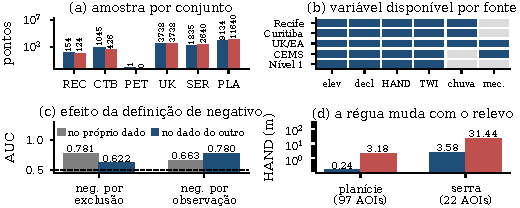
\includegraphics[width=0.97\columnwidth]{fig/fig2_datasets.pdf}
\caption{Quatro desafios, nos dados reais do projeto. (a) pontos por conjunto
(SER e PLA: AOIs de serra e planície do EMS). (b) HAND em Recife sob negativo por
ausência: classes sobrepostas. (c) cada modelo no próprio dado e no do outro: o
de maior AUC próprio é o que menos transfere. (d) HAND por classe de relevo.}
\label{fig:datasets}
\end{figure}

% ------------------------------ TABELA I ------------------------------
\begin{table*}[!t]
\caption{Resumo de materiais e métodos; a Seção~II contextualiza cada linha.}
\label{tab:mm}
\centering
\renewcommand{\arraystretch}{0.95}
\scriptsize
\begin{tabular}{@{}>{\raggedright\arraybackslash}p{2.05cm}>{\raggedright\arraybackslash}p{7.6cm}>{\raggedright\arraybackslash}p{6.5cm}@{}}
\toprule
\textbf{Materiais} & \textbf{Descrição} & \textbf{Observações} \\
\midrule
Rótulo &
Positivos: SEDEC/Recife (154), SIAC 156/Curitiba (1.045), Diário Oficial,
ANA/SNIRH, Global Flood Database~\cite{tellman2021}. Negativo \emph{observado}:
Copernicus EMS, 25.249 pontos em 119 AOIs, mais a ativação EMSR720 no Rio Grande do
Sul (216,55\,km$^2$; 5,94:1). Negativo por \emph{exclusão qualificada}: Environment
Agency/UK, 7.476 pontos (3.738/3.738) em 201 eventos independentes &
Três níveis declarados por linha. Nenhuma região brasileira tem o nível de
observação; o portão de negativo formal segue aberto para as três. \\
Bases, variáveis e modelos &
MDT PE3D 10\,m, Copernicus DEM GLO-30 e SGB/CPRM; CHIRPS~\cite{funk2015} e
ERA5-Land~\cite{munoz2021}; Sentinel-1/2 e cobertura do solo (auxiliares). Elevação,
declividade, HAND~\cite{renno2008} e TWI~\cite{beven1979} por D-infinity~\cite{tarboton1997};
pico e decaimento de chuva. Firth~\cite{firth1993} como rota primária e GBM/GAM/EBM como
diagnóstico; \emph{gate} EPV~\cite{peduzzi1996}, \emph{bootstrap} de grupos $N$\,=\,1000,
validação agrupada por evento ou AOI e \emph{walk-forward} &
Nenhuma variável derivada do rótulo, de escore ou de limiar; as orbitais \textbf{não
são causais}. Chuva só existe no piloto inglês: o modelo multirregião roda com quatro
variáveis. A rota primária segue linear mesmo quando o não linear tem AUC maior. \\
Produto, ambiente e recursos &
API FastAPI com contrato de inferência e geoprocessamento sob demanda; \emph{model
card}~\cite{mitchell2019}; camada LLM. Python 3.10 com \texttt{firthlogist},
\texttt{scikit-learn}, \texttt{interpret}, \texttt{rasterio}/GDAL, \texttt{whitebox} e
\texttt{pytest}; estação de 10 núcleos e 15,5\,GB, sem GPU; QGIS 3, GEE, Git &
A LLM lê o \emph{payload} já decidido. Recursos medidos: Firth 0,056\,s, EBM 25,3\,s. \\
\bottomrule
\end{tabular}
\end{table*}

% =====================================================================
\section{Etapas do Projeto e Marcos Físicos}
\label{sec:etapas}

Cada etapa é encerrada por um arquivo conferível, produzido antes de a seguinte
começar; as datas da disciplina (Seção~\ref{sec:crono}) sincronizam, mas não
substituem esse critério.

\textbf{E0 e E1 --- Base consolidada e escopo congelado (concluídas).} Corpus,
governança de \emph{claims}, teste de ablação e definição de qual documento rege
o trabalho. \emph{Evidência}: artefatos versionados, os três valores de acurácia
balanceada e uma afirmação de estado por arquivo.

\textbf{E2 --- Conjunto de treino com negativo observado (M1).} Consolidar as
fontes de negativo numa tabela única, com nível de negativo, unidade de
agrupamento e classe de relevo carimbados por linha. \emph{Entregável}: conjunto
de treino multirregião. \emph{Evidência}: contagem por classe, por nível e por
grupo; nenhum ponto sem unidade de agrupamento.

\textbf{E3 --- Estimação e validação agrupada (M2).} Ajustar o modelo por classe
de relevo, com validação agrupada e aplicação cruzada entre fontes de negativo.
\emph{Entregável}: tabelas de coeficientes com intervalo e de desempenho por
classe. \emph{Evidência}: EPV verificado antes de cada ajuste, sinais físicos
conferidos depois, nenhum ajuste após olhar o teste.

\textbf{E4 --- \emph{Holdout} temporal sobre os eventos externos (M3).} É o teste
mais forte ainda não realizado e não exige aquisição nova: os eventos do piloto
inglês se distribuem em cerca de 158 datas ao longo de 25 anos.
\emph{Entregável}: desempenho por corte. \emph{Evidência}: cortes definidos
antes da execução.

\textbf{E5 --- Camada de explicação sobre o contrato (M4).} Testar a LLM sobre
respostas reais da API, inclusive as de recusa. \emph{Entregável}: cenários com
resposta estruturada e explicação. \emph{Evidência}: nenhuma explicação
contradiz o \emph{payload} nem preenche escore ausente.

\textbf{E6 e E7 --- Congelamento, redação e pôster (M5--M7).} Testes completos,
repositório limpo e \emph{tag} de congelamento; depois dessa data, apenas redação
sobre artefatos congelados. \emph{Evidência}: cada número do manuscrito
rastreável a um arquivo.

\textbf{Riscos e rotas alternativas.} Declaradas agora, não improvisadas depois.
Em E2, se o pareamento entre fontes com e sem chuva não for alcançável, o piloto
inglês vira conjunto de sensibilidade e o modelo conjunto roda só com terreno. Em
E4, se o desempenho temporal não superar o acaso, o resultado é publicado como
está. Em E5, se a explicação divergir do \emph{payload}, a camada vira gerador de
texto por regras sobre os mesmos campos. Nenhuma delas altera a pergunta de
pesquisa.

% =====================================================================
\section{Cronograma}
\label{sec:crono}

O cronograma (Tabela~\ref{tab:crono}) cobre da submissão deste plano à
apresentação final e incorpora os \emph{checkpoints} da disciplina. O estado da
arte já está em curso e permanece ativo até a redação. Sendo o trabalho
individual, as etapas não correm em paralelo entre pessoas, mas se sobrepõem no
tempo; foram identificadas de antemão sem que a ordem de conclusão seja
obrigatória --- o que muda de posição é a etapa, nunca o critério de evidência
que a encerra --- e a distribuição prevê folga porque pesquisa costuma exceder o
prazo estimado. Os intervalos de 08/09 e 13/10 seguem sem tarefa nova; 24/11 e
01/12 são contingência.

\begin{table}[!h]
\caption{Cronograma (quinzenas). E01 29/08, E02 31/10, E03 09/11, defesa 17/11.}
\label{tab:crono}
\centering
\renewcommand{\arraystretch}{0.88}
\setlength{\tabcolsep}{2.6pt}
\tiny
\begin{tabular}{@{}>{\raggedright\arraybackslash}p{1.95cm}ccccccc@{}}
\toprule
\textbf{Atividade} & \textbf{09--29} & \textbf{01--15} & \textbf{16--29} &
\textbf{30/09--} & \textbf{14--31} & \textbf{01--09} & \textbf{10--17} \\
 & \textbf{ago} & \textbf{set} & \textbf{set} & \textbf{13/10} &
\textbf{out} & \textbf{nov} & \textbf{nov} \\
\midrule
Estado da arte          & X & X & X &   &   &   &   \\
Dados (E2)              & X & X &   &   &   &   &   \\
Experimentação (E3--E4) &   & X & X &   &   &   &   \\
Produto/LLM (E5)        &   &   & X & X &   &   &   \\
Análise                 &   &   & X & X & X &   &   \\
Auditoria (E6)          &   &   &   & X &   &   &   \\
Redação (E7)            &   &   &   & X & X & X &   \\
Pôster e defesa         &   &   &   &   &   & X & X \\
\midrule
\textit{Checkpoints} & \textbf{E01} & & & & \textbf{E02} & \textbf{E03} & \textbf{Def.} \\
\bottomrule
\end{tabular}
\end{table}

% =====================================================================
\fontsize{5.7}{6.2}\selectfont
\begin{thebibliography}{99}
\setlength{\itemsep}{0.4pt}
\setlength{\parskip}{0pt}

\bibitem{tellman2021}
B. Tellman \emph{et al.}, ``Satellite imaging reveals increased proportion of
population exposed to floods,'' \emph{Nature}, vol. 596, pp. 80--86, 2021.

\bibitem{renno2008}
C. D. Rennó \emph{et al.}, ``HAND, a new terrain descriptor using SRTM-DEM:
Mapping terra-firme rainforest environments in Amazonia,''
\emph{Remote Sensing of Environment}, vol. 112, no. 9, pp. 3469--3481, 2008.

\bibitem{beven1979}
K. J. Beven and M. J. Kirkby, ``A physically based, variable contributing area
model of basin hydrology,'' \emph{Hydrological Sciences Bulletin}, vol. 24,
no. 1, pp. 43--69, 1979.

\bibitem{tarboton1997}
D. G. Tarboton, ``A new method for the determination of flow directions and
upslope areas in grid digital elevation models,'' \emph{Water Resources
Research}, vol. 33, no. 2, pp. 309--319, 1997.

\bibitem{li2022pul}
W. Li \emph{et al.}, ``A positive-unlabeled learning algorithm for urban flood
susceptibility modeling,'' \emph{Land},
vol. 11, no. 11, art. 1971, 2022.

\bibitem{agostini2024}
G. Agostini, E. Pierson, and N. Garg, ``A Bayesian spatial model to correct
under-reporting in urban crowdsourcing,'' in \emph{Proc. AAAI}, vol. 38, 2024,
pp. 21\,888--21\,896.

\bibitem{firth1993}
D. Firth, ``Bias reduction of maximum likelihood estimates,''
\emph{Biometrika}, vol. 80, no. 1, pp. 27--38, 1993.

\bibitem{peduzzi1996}
P. Peduzzi \emph{et al.}, ``A simulation study of the number of events per
variable in logistic regression analysis,'' \emph{J. Clin. Epidemiol.}, vol. 49,
no. 12, pp. 1373--1379, 1996.

\bibitem{funk2015}
C. Funk \emph{et al.}, ``The climate hazards infrared precipitation with
stations,'' \emph{Scientific Data}, vol. 2, art. 150066, 2015.

\bibitem{munoz2021}
J. Muñoz-Sabater \emph{et al.}, ``ERA5-Land: a global reanalysis dataset for land
applications,'' \emph{Earth Syst. Sci. Data}, vol. 13, pp. 4349--4383, 2021.

\bibitem{mitchell2019}
M. Mitchell \emph{et al.}, ``Model cards for model reporting,'' \emph{Proc. ACM
FAT*}, pp. 220--229, 2019.

\end{thebibliography}

\end{document}
